%%%%%%%%%%%%%%%%%%%%%%%%%%%%%%%%%%%%%%%%%%%%%%%%%%%%%%
%SEC%%%%%%%%%%%%%%%%%%%%%%%%%%%%%%%%%%%%%%%%%%%%%%%%%%
\section{Conclusões}

%FRAME%%%%%%%%%%%%%%%%%%%%%%%%%%%%%%%%%%%%%%%%%%%%%%%
\begin{frame}{Conclusões}
\begin{itemize}
    \item O algoritmo de Viola-Jones é eficiente para detectar faces
    \item A biblioteca OpenCV possui diversos algoritmos implementados e facilita o desenvolvimento de aplicações
    \item A taxa de acertos do Eigenfaces é baixa quando comparada a outros métodos
    \item Reconhecimento facial irrestrito ainda é um desafio por fatores como iluminação, baixa resolução, variação de pose, oclusão e expressão facial
    \item Soluções comerciais, como a Face API da Microsoft, oferecem o estado da arte em diversas tarefas como detecção facial, reconhecimento facial, detecção de emoções e identificação de gênero
    \item É possível utilizar o Raspberry Pi como uma solução barata de câmera inteligente
\end{itemize}
\end{frame}


%FRAME%%%%%%%%%%%%%%%%%%%%%%%%%%%%%%%%%%%%%%%%%%%%%%%
\begin{frame}{Trabalhos Futuros}
\begin{itemize}
    \item Treinar um classificador com menos falso-positivos
    \item Estudar novos métodos de reconhecimento facial e extração de características para substituir a Face API da Microsoft
\end{itemize}
\end{frame}


%FRAME%%%%%%%%%%%%%%%%%%%%%%%%%%%%%%%%%%%%%%%%%%%%%%%
\begin{frame}{Trabalhos Futuros}
\begin{itemize}
    \item Criar um dashboard com gráficos e tabelas que facilitem a tomada de decisões utilizando as informações coletadas
\end{itemize}
\begin{figure}[htbp]
%    \caption{Teste da Microsoft Face API}
    \label{fig:tableau}
    \centering
    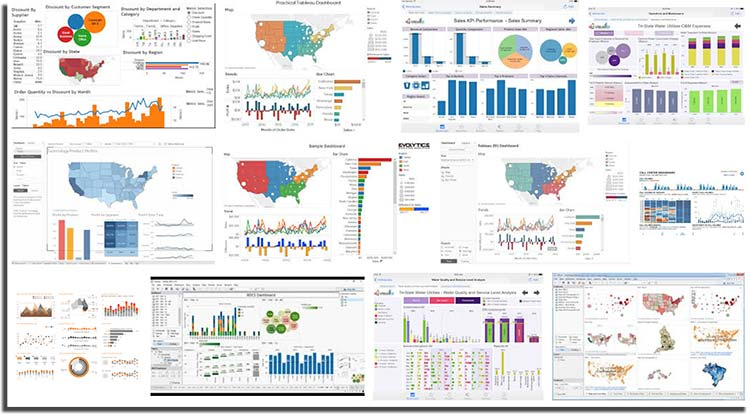
\includegraphics[height=0.7\textheight,width=\textwidth,keepaspectratio]{imagens/tableau.jpg}
\end{figure}
\end{frame}